\section{Introduction}

This manuscript records a bounded finite theorem package for a 900-vertex graph candidate in the Thalean program. The aim is deliberately narrow. We do not attempt to prove uniqueness among all possible 900-vertex constructions, identify the graph in an external census, or attach a physical interpretation. The purpose is to admit one explicit generated candidate by a finite kernel and a closed certificate ledger.

The workflow separates three layers.

\begin{enumerate}[leftmargin=2em]
\item The construction kernel defines the finite input data and generation law.
\item The proof kernel records which consequences follow directly from the kernel and which require certificates.
\item The admission ledger closes when every load-bearing claim is either proved by the kernel or certified by a finite, reproducible check.
\end{enumerate}

The result is a receipted theorem package: the object is generated, checked, compared, and bounded by explicit negative claims.

After the bounded graph-admission theorem, the paper also records a separate local overlay audit. That audit concerns a WXYZTI reciprocal pair grammar over realized station rows. It is included as a certificate-backed witness structure, not as an additional premise of the main theorem. The distinction matters: the graph \(X_\sigma\) is admitted by the kernel and graph certificates, whereas the WXYZTI section records a bounded local grammar whose native generator remains open.




\begin{center}
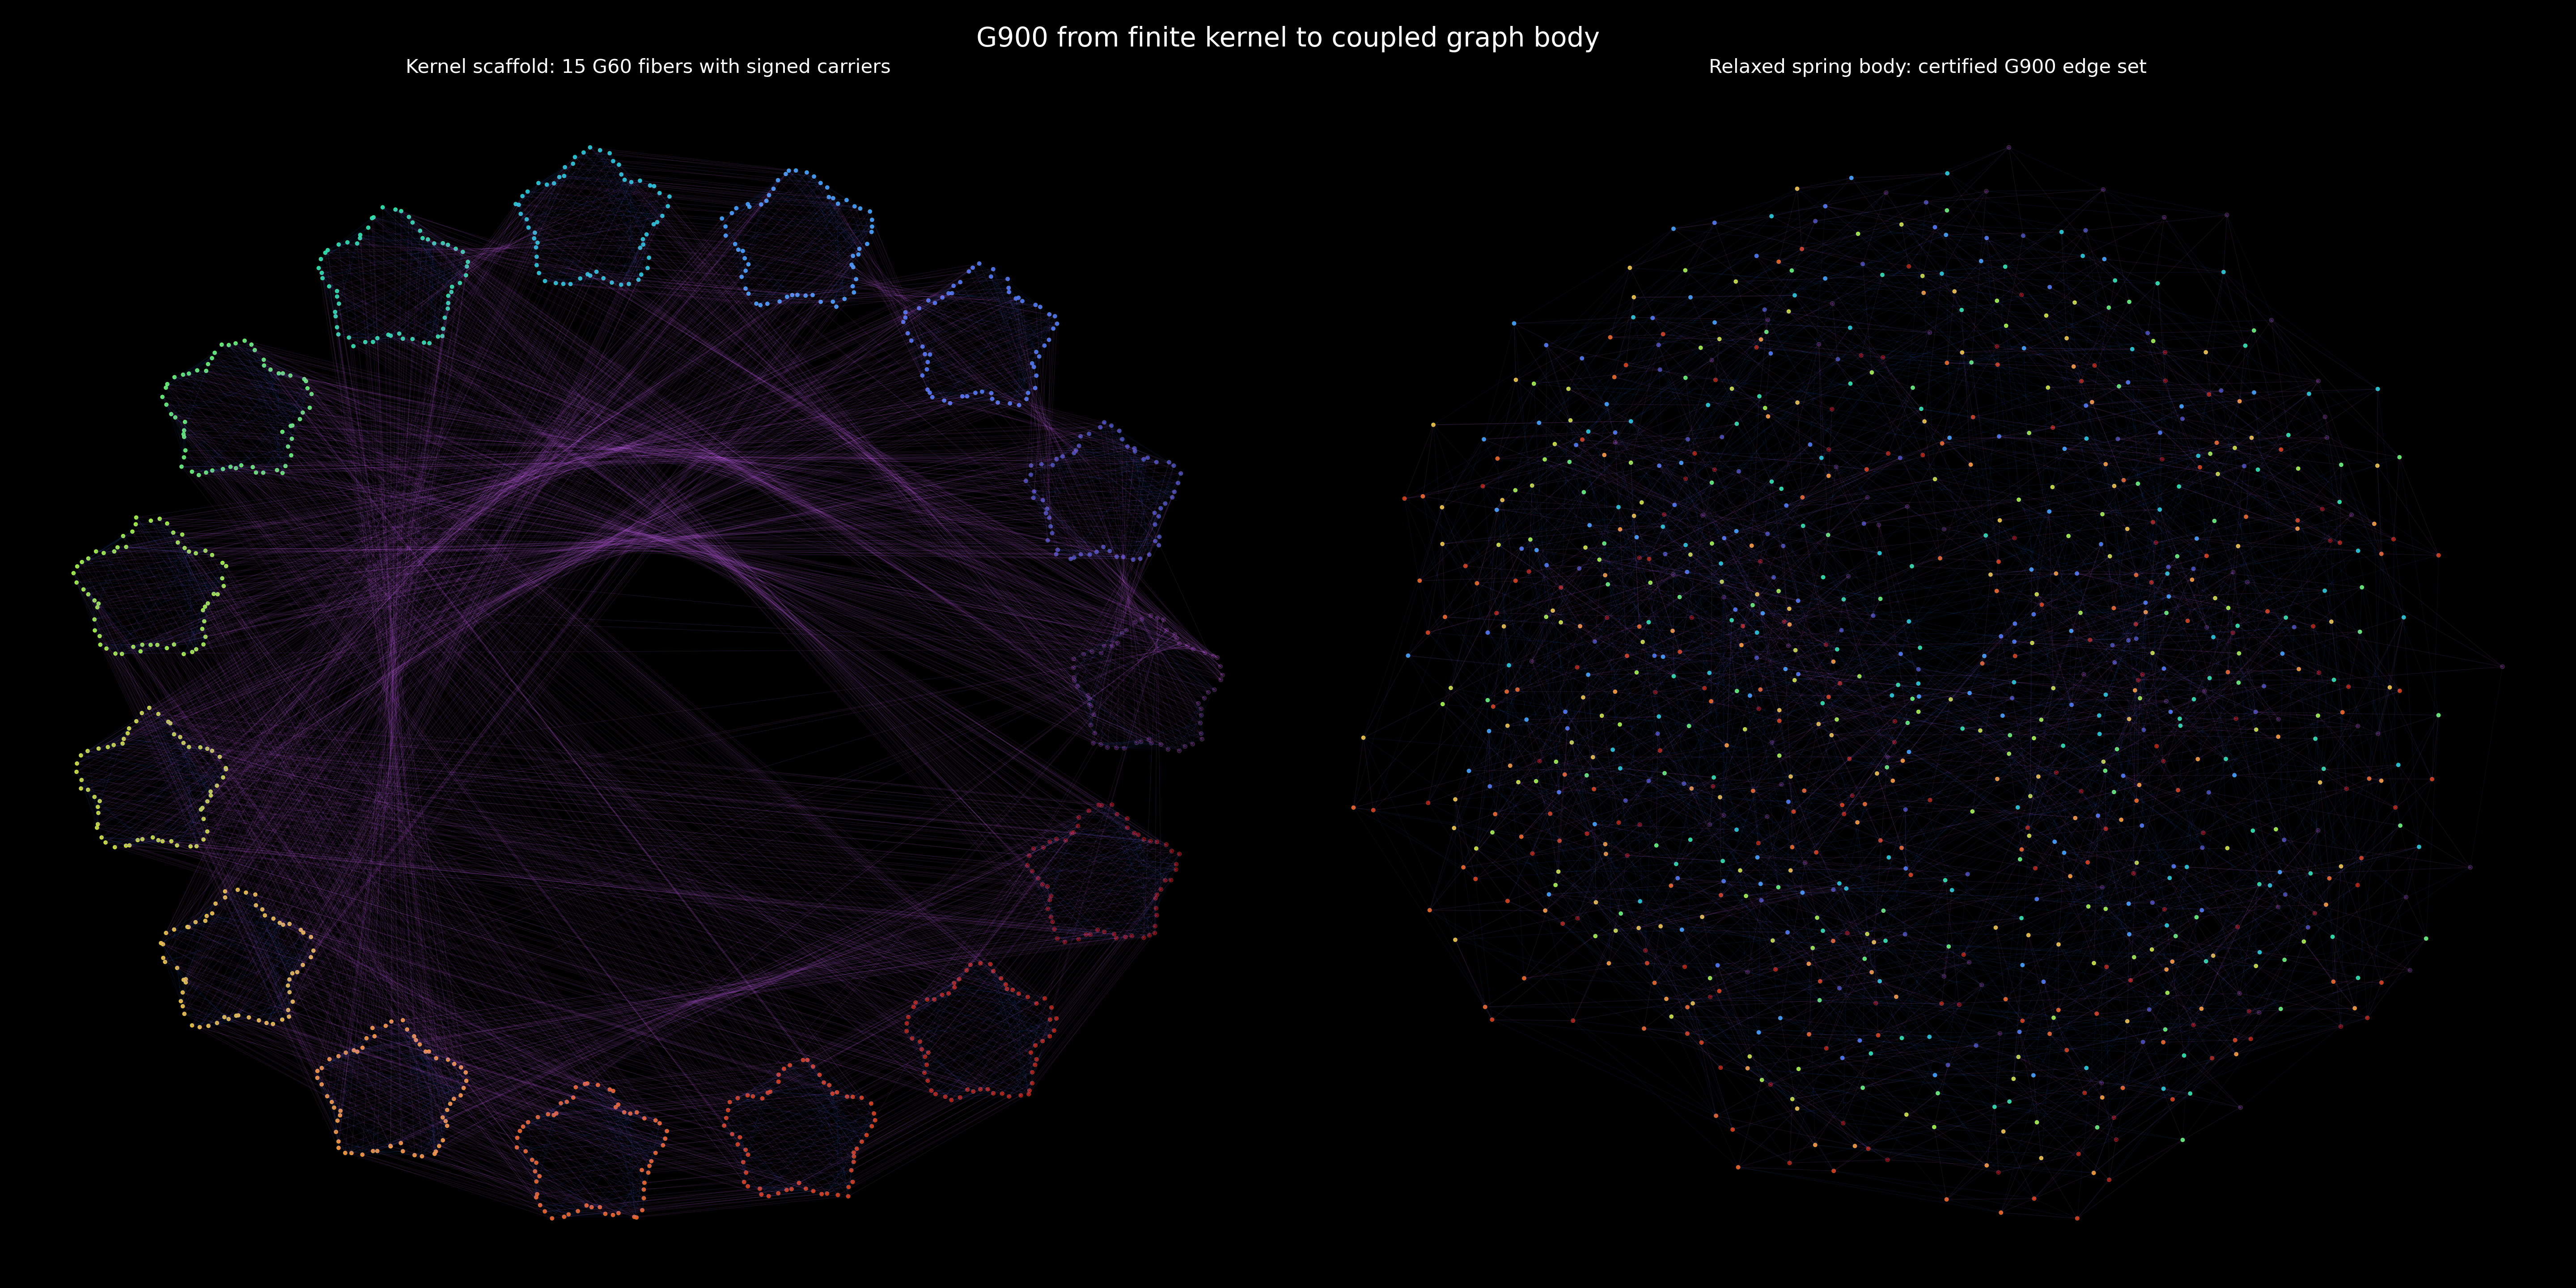
\includegraphics[width=\textwidth]{figures/g900_scaffold_vs_spring.png}

\small
\textbf{Figure 1.} Two views of the certified Project 18 edge set. Left: the finite construction scaffold, showing fifteen \(G_{60}\) fibers coupled by signed carriers. Right: the relaxed spring body of the same 900-vertex, 3600-edge graph. The figure is illustrative; the theorem rests on the finite kernel and certificates.
\end{center}


